% Chapter Template

\chapter{Fundamental Definitions and Examples.} % Main chapter title

\label{Chapter 1} % Change X to a consecutive number; for referencing this chapter elsewhere, use \ref{ChapterX}

%% to include section files use the \input{} command.

The goal of matroid theory is to provide an abstract theory of independence.
Matroids have their roots in algebra (especially linear algebra), graph theory,
and combinatorics; and each field provides a distinct flavor to the subject. The
notion of independence was first covere by Whitney in $1935$, and then Van der
Waerden, in $1937$, in his seminal work ``Moderne Algebra''. Gian Carlo Rota
would also stumble upon the theory indepednetly. Pioneering work would later be
done by Tutte, Nakasawa, Birkhoff, and Mac Lane.

Perhaps the most important aspect of matroids is that they have several
equivalent definitions. We begin by studying two of them.

%----------------------------------------------------------------------------------------
%	SECTION 1.1
%----------------------------------------------------------------------------------------

\section{More on Polynomial Rings.}
\label{section1}

\begin{definition}
    Let $R$ be a commutative ring with identity $1 \neq 0$, and $I$ an ideal of
    $R$. Then
    \begin{equation*}
        \faktor{R[x]}{I[x]} \simeq \faktor{R}{I}[x]
    \end{equation*}
    That is, the factor ring of the polynomial rings is isomorphic to the
    polynomial ring of the factor ring.
\end{definition}

%----------------------------------------------------------------------------------------
%	SECTION 1.1
%----------------------------------------------------------------------------------------

\section{Connected Spaces of The Real Line.}

\begin{definition}
    We call a simply ordered set $L$ with  $|L|>1$ a  \textbf{ordered contunuum} if:
        \begin{enumerate}[label=(\arabic*)]
            \item $L$ has the least upperbound property.

            \item If $x<y$, then there exists a  $z$ such that  $x<z<y$.
        \end{enumerate}
\end{definition}

\begin{theorem}\label{3.2.1}
    If $L$ is a linear continuum in the order topology, then  $L$ is connected, and so are the open
    sets of  $L$  (the intervals and rays in $L$).
\end{theorem}
\begin{proof}
    We show that convex sets are connected. Let $Y=A \cup B$ be a seperation, and choose  $a \in A$,
     $b \in B$ with  $a<b$. We have that the interval of points in  $L$,  $[a,b] \subseteq Y$; and
     we also have that $[a,b] \subseteq A_0 \cup B_0$ with $ A_0=A \cap [a,b]$ and $ B_0=B \cap
     [a,b]$. Now $ A_0,B_0 \neq \emptyset$, so $[a,b]=A_0 \cup B_0$ is a seperation of $[a,b]$. Now
     let $c=\sup{A_0}$. Suppose first that $c \in B_0$, then $c \neq a$, so either $c=b$ or  $a<c<b$.
     Since  $ B_0$ is open in $[a,b]$ as a subspace of $Y$, there is some interval  $(d,c] \subseteq
     B_0$.

     If $c=b$, then  $d<c$ is an upperbound of  $ A_0$, which contradicts that $c$ is the least
     upperbound. Now suppose that $c<b$. We have that since  $c,b \in B_0$, $(c,b] \cap A_0=
     \emptyset$, then $(b,d] \cap A_0=(d,c] \cap (c,b] \cap A_0 = \emptyset$, and again we have
     $d<c$ which gives us the contradiction. So  $c \notin B$. By similar reasoning  $c \notin A_0$.
\end{proof}
\begin{corollary}
    $\R$ is connected and so are the intervals and rays of  $\R$.
\end{corollary}
\begin{proof}
    $\R$ is a linear continuum.
\end{proof}

\begin{theorem}[The Intermediate Value Theorem]\label{3.2.2}
    Let $f:X \rightarrow Y$ be continuous with  $X$ connected, and  $Y$ an ordered set under the
    order topology. If  $a,b \in X$, and if  $r \in Y$ such that  $f(a)<r<f(b)$ or $f(b)<r<f(a)$,
    then there exists a $c \in X$ for which  $f(c)=r$.
\end{theorem}
\begin{proof}
    Let $r \in Y$ such that  $f(a)<r<f(b)$, without loss of generality. We have that $A=f(X) \cap
    (-\infty, r)$ and $B=f(X) \cap (r ,\infty)$ are disjoint, nonempty sets open if $f(X)$ as a
    subspace of $Y$. Now suppose there is no  $c \in X$ for which  $f(c)=r$, then $f(X)=A \cup B$ is
    a seperation of $f(X)$, which contradicts theorem \ref{3.1.6}.
\end{proof}

\begin{example}
    \begin{enumerate}[label=(\arabic*)]
        \item The ordered square $I_0^2$ is a linera continuum. Let $A \subseteq I_0^2$ and consider
            the projection $\pi_1:I_0^2 \rightarrow I_0^2$. Let $b=\sup{\pi_1(A)}$, now if $b \in
            \pi_1(A)$ then $A \cap (b \times I_0) \neq \emptyset$, and since $I_0 \subseteq \R$, $A
            \cap (b \times I_0)$ has a least upperbound, $b \times c$, where  $c=\sup{I_0}$, which
            is also the least upperbound of $A$. Now if we have $a \times c < b \times d$, then
            $a<b$ and  $c<d$; and since  $\R$ is a linear continuum, there are $y,z \in \R$ for
            which  $a<y<b$ and  $c<z<d$. Hence  $a \times c < y \times z < b \times d$; which makes
            $ I_0^2$ into a liear continuum.

        \item If $X$ is a well ordered set, then  $X \times [0,1)$ is a linear contiuum in the
            dictionary order. Let $A \subseteq X \times [0,1)$ and consider the projection $\pi_2:X
            \times [0,1) \rightarrow [0,1)$. If $b=\sup{\pi_2(A)}$, then $A \cap (b \times [0,1)) \neq
            0$, and so $A \cap (b \times [0,1)$ has a least upperbound $b \times c$ with
            $c=\sup{[0,1)}$, which is also a least upperbound of $A$.

            Now since $\R$ is a linear continuum, if $x \times a < y \times b$, under the dictionary
            order, then  $x \leq y$ and  $a<b$. Then there are  $c,z \in \R$ such that  $x \leq z
            \leq y$ and  $a<c<b$, so that $x \times a < z \times c < y \times b$.
    \end{enumerate}
\end{example} 

\begin{definition}
    Let $X$ be a topological space with  $x, y \in X$. A \textbf{$xy$-path} in $X$ from  $x$ to  $y$ is a
    continuous map  $f:[a,b] \rightarrow X$, with $[a,b] \subseteq \R$ such that $f(a)=x$, and
    $f(b)=y$. We call $X$ \textbf {path connected} if there exists an $xy$-path in $X$ for every
    $x,y \in X$.
\end{definition}

\begin{theorem}\label{3.2.3}
    Path connected spaces are connected
\end{theorem}
\begin{proof}
    Let $X$ be path connected, and suppose that  $X=A \cup B$ is a seperation of  $X$. Let  $f:[a,b]
    \rightarrow X$ be some path in $X$. Since  $f$ is continuous, and  $[a,b] \subseteq \R$, by
    theorem \ref{3.1.6}, $f([a,b]) \subseteq X$ is a connected subspace, so either $f([a,b])
    \subseteq A$ or $f([a,b]) \subseteq B$, so there is no path from a point in $A$ to a point in
    $B$. But  $X$ is path connected; a contradiction. Therefore  $X$ must be connected.
\end{proof}

\begin{example}
    \begin{enumerate}[label=(\arabic*)]
        \item Define the \textbf{unit ball} in $\R^n$ under  $||\cdot||$ to be  $B^n=\{x \in
            \R^n:||x|| \leq 1\}$. $B^n$ is path connected. Consider  $f[0,1] \rightarrow B^n$ by
            $f(t)=(1-t)x+ty$, then $||f(t)||=(1-t)||x||+t||y|| \leq 1$, hence $f(t) \in  B^n$.
            Extending this to arbitrariy balls, for $\epsilon>0$, $B(x,\epsilon)$ and
            $cl{B(x,\epsilon)}$ are also path connected. The function $f$ also shows that the unit
            ball, and open balls  (as well as their closure) are convex.

        \item Define \textbf{punctured Euclidean space} to be $\com{\R^n}{\{0\}}$. If $n>1$,
        $\com{\R}{\{0\}}$ is path connected. Connect the points $x,y \in \com{\R^n}{\{0\}}$ by a
        straight line not passing through $0$, or choose a point $z \in \com{\R^n}{\{0\}}$ on that
        line and form a path by adjoining the lines from $x$ to  $z$ and from  $z$ to  $y$

        \begin{figure}[h] 
            \centering
            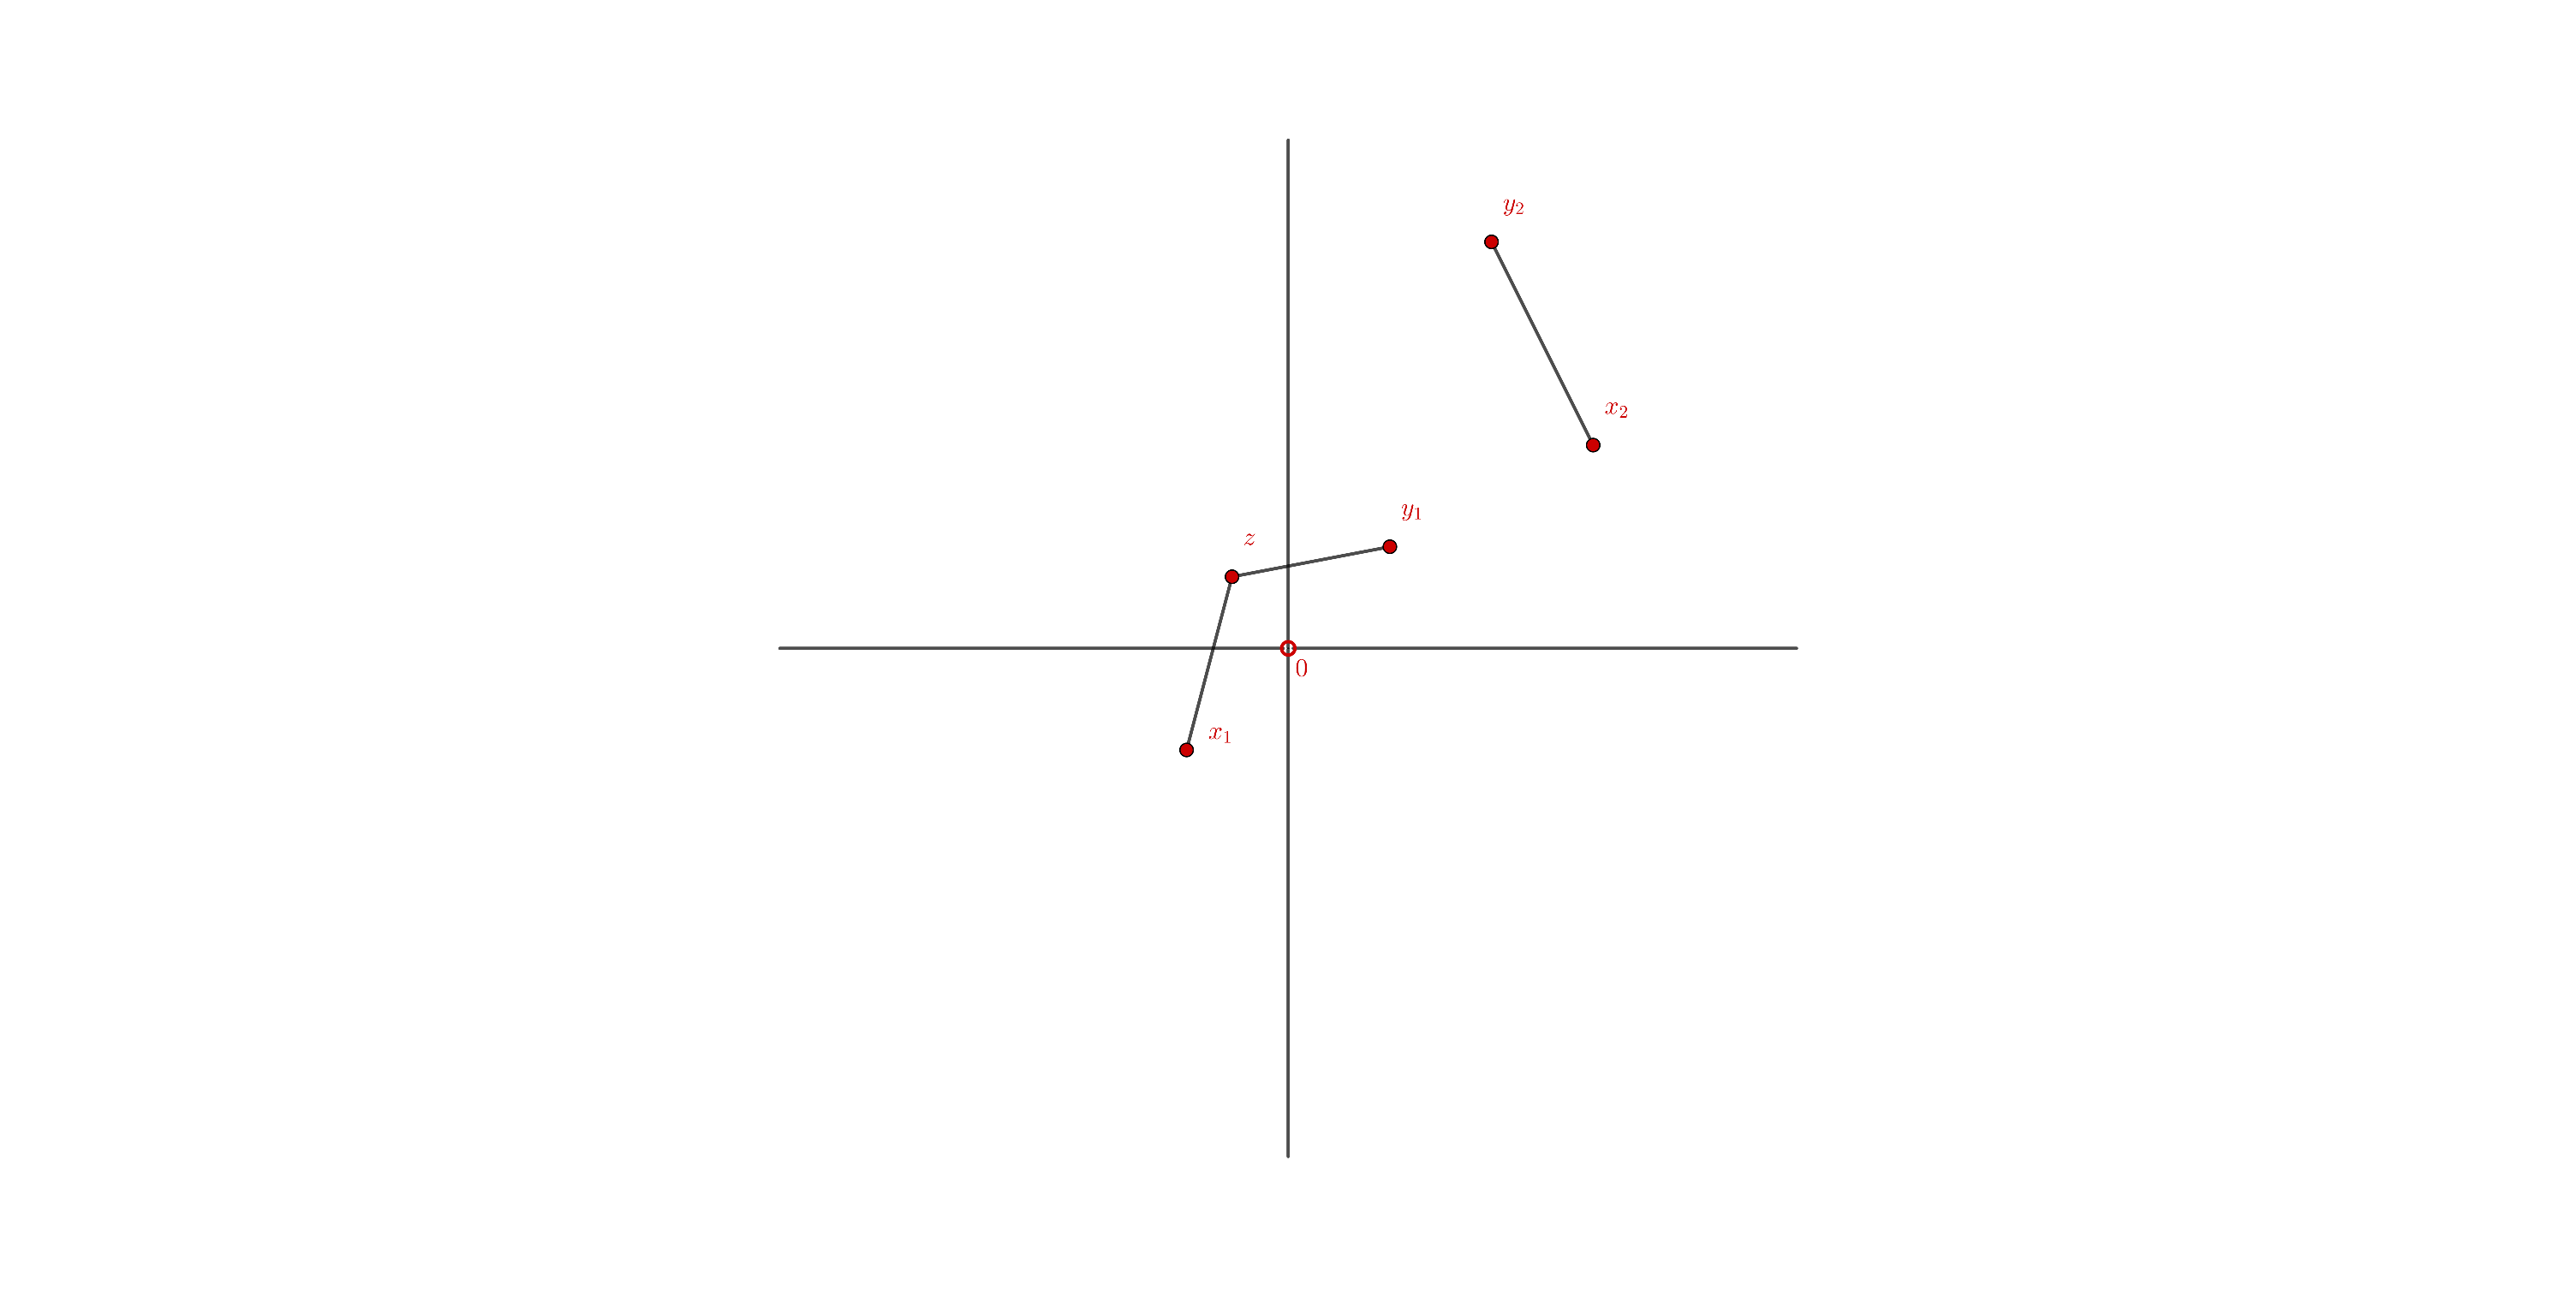
\includegraphics[scale=0.2]{Figures/Chapter3/puncturedSpace.eps}
            \caption{Punctures $2$-space $\com{\R^2}{\{0\}}$.}
            \label{fig_3.1}
        \end{figure}

    \item Consider the unit sphere $S^{n-1}=\{x \in \R^n:||x||=1\}$ in $\R^n$.  $S^{n_-1}$ is path
        connected for $n>1$. Take the map  $g:\com{\R^n}\{0\} \rightarrow S^{n-1}$ by $g:x
        \rightarrow \frac{x}{||x||}$.

    \item The ordered square $ I_0^2$ is connected, but it is not path connected/ Let $p=0 \times
        0$,  $1=1 \times 1$ and let  $f:[a,b] \rightarrow I_0^2$ be a path joining $p$ and  $q$. We
        have that  $f([a,b])$ must contain all $x \times y \in I_0^2$ by the intermediate value
        theorem. Hence for each  $x \in I_0$, $U_x=f^{-1}(x \times I_0) \neq \emptyset$ and it is
        also open in $[a,b]$. Now choose for each $x \in I_0$, $q_x \in \Q$ such that  $q_x \in
        U_x$. Since  $\bigcap_{x \in I_0}{U_x} = \emptyset$, the map $x \rightarrow q_x$ is  $1-1$
        of  $I_0$ onto $\Q$. which makes $I_0$ countable; a contradiction.

    \item 
        \begin{figure}[h]
            \centering
            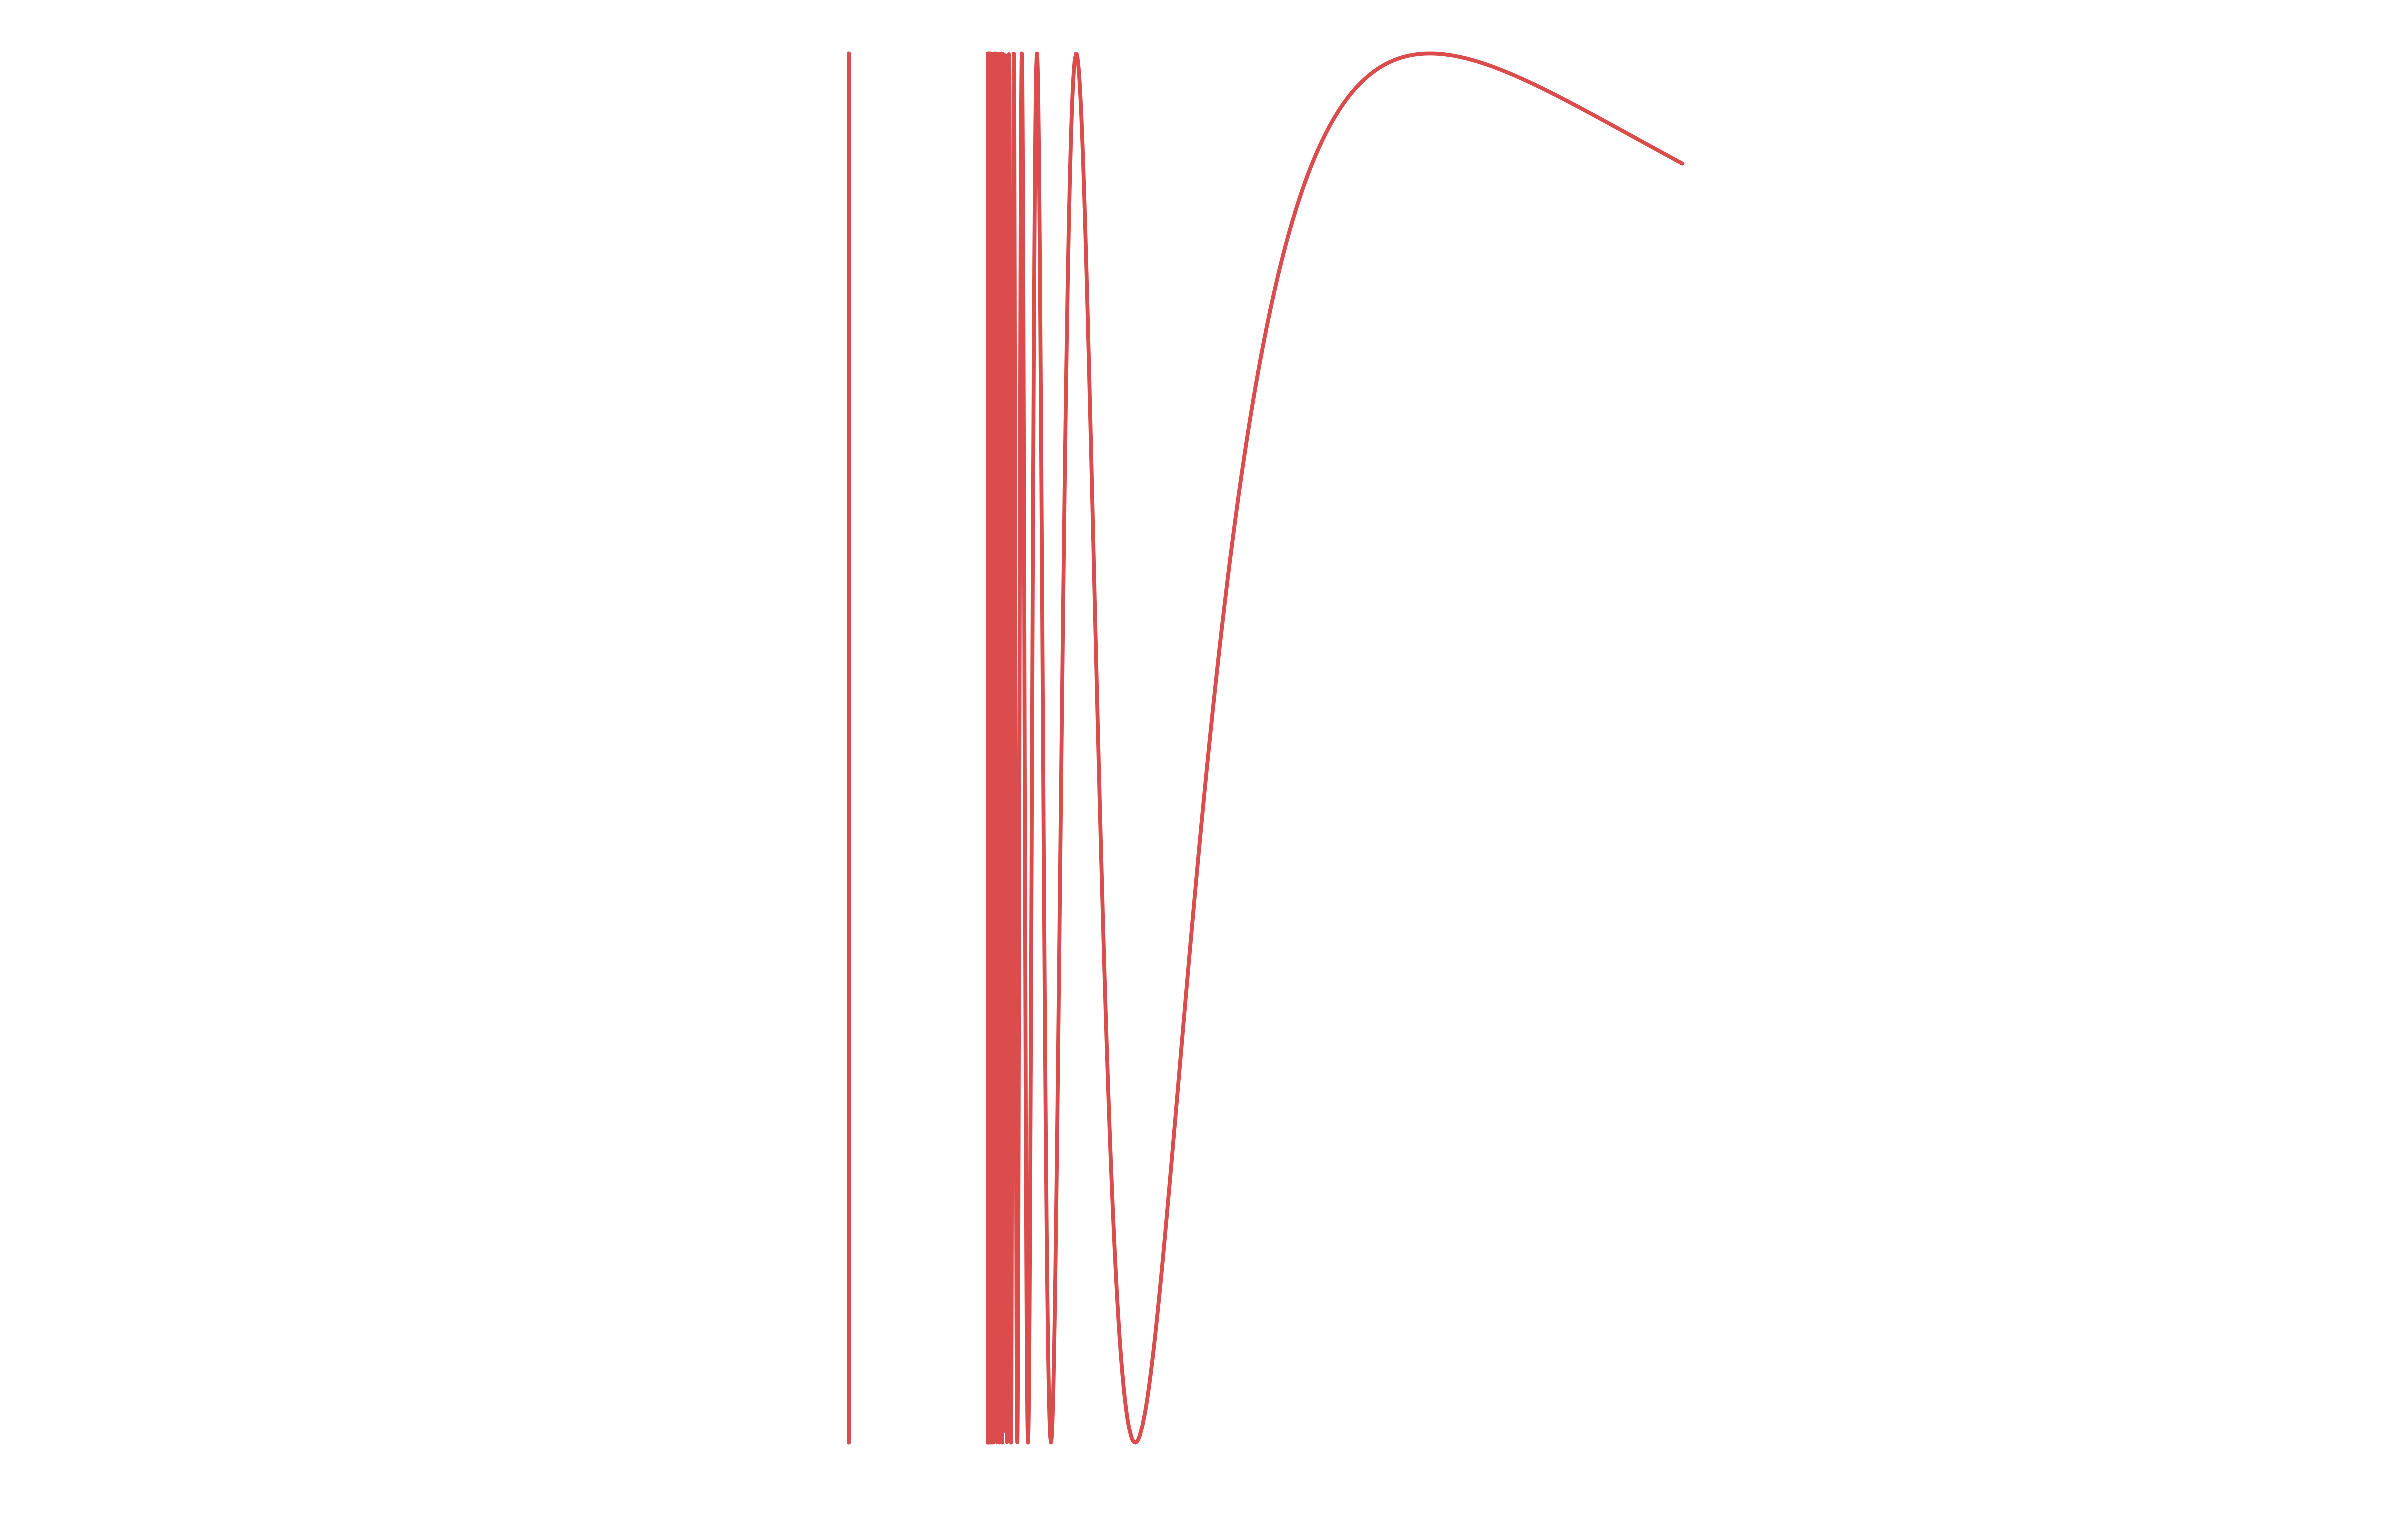
\includegraphics[scale = 0.2]{Figures/Chapter3/topologistsSineCurve.eps}
            \caption{The topologists Sine Curve, defined by $x \times \sin{\frac{1}{x}}$.}
            \label{fig_3.2}
        \end{figure}

        Let $S=\{x \times \sin{\frac{1}{x}}:0 < x \leq 1\}$. This is the image of the continuous map
        $x \rightarrow x \times \sin{\frac{1}{x}$ from $(0,1] \rightarrow \R^2$, Since $(0,1]$ is
            connected, then so is $S$. by theorem \ref{3.1.6}. We call $\cl{S}=S \cup (0 \times
            [-1,1])$ the \textbf{topologist's sine curve} (see figure \ref{fig_3.2}).

            Suppose that $f:[a,c] \rightarrow \cl{S}$ is a path begining at $0$ and ending at a
            point in  $S$. The set  $T=\{t \in \R:f(t) \in 0 \times [-1,1]\}$ is closed, so it has a
            largest element $b$. Then  $f$ is a path mapping  $b \rightarrow 0 \times [-1,1]$ and
            taking all other points to $S$. Suppose that  $[b,c]=[0,1]$ and let $f(t)=(x(t),y(t))$
            where $x(0)=0$, $x(t)>0$ and $y(t)=\sin{\frac{1}{x(t)}}$ for all $t>0$. For  $n \in
            \Z^+$, choose  $0<u<x(\frac{1}{n})$ such that $\sin{\frac{1}{u}}=(-1)^n$. By the
            intermediate value theorem, there are $0<t_n<\frac{1}{n}$ with $x(t_n)=u$. Then the
            sequence $\{t_n\} \rightarrow 0$, and $x(t_n)=(-1)^n$, which diverges; a contradiciton
            since $x(0)=0$ and $\{t_n\} \rightarrow 0$. Hence $\cl{S}$ is not path connected.

    \end{enumerate}
\end{example} 

\section{Outer Measures}

\begin{definition}
    Let $X$ be a set. An \textbf{outer-measure} on $X$ is a function $m^\ast:2^X
    \xrightarrow{} [0, \infty)$ for which the following are true:
    \begin{enumerate}
        \item[(1)] $m^\ast(\emptyset)=0$.

        \item[(2)] If $A \subseteq B$, then $m^\ast(A) \leq m^\ast(B)$.

        \item[(3)] If $\{A_n\}$ is a countable collection of subsets of $X$,
            then
            \begin{equation*}
                m^\ast\Big{(} \bigcup{A_n} \Big{)} \leq \sum{m^\ast(A_n)}
            \end{equation*}
    \end{enumerate}
\end{definition}

\begin{lemma}\label{lemma_1.3.1}
    Let $X$ be a set, and  $\Ec$ a collection of subsets of $X$ for which
    $\emtyset \in \Ec$ and $X \in \Ec$, and let $l:\Ec \xrightarrow{} [0, \infty]$
    a function for which $l(\emptyset)=0$. For any $A \subseteq X$, define
    \begin{equation}\label{equation_1.4}
        m^\ast(A)=\inf{\Big{\{} \sum{l(E_n)} : E_n \in \Ec, \text{ and }
       A \subseteq \bigcup{E_n} \Big{\}}}
    \end{equation}
    Then $m^\ast$ defines an outer-measure.
\end{lemma}
\begin{proof}
    For all $A \subseteq X$, there is a collection $\{E_n\}$ of sets of $\Ec$
    for which $A \subseteq \bigcup{E_n}$. Observe first, that since $l(E_n) \geq
    0$ for all $n$, that  $\sum{l(E_n)} \geq 0$. This makes $m^\ast(A) \geq 0$.
    Now, choose $E_n=\emptyset$ for all  $n$, and we get  $m^\ast(\emptyset)=0$.

    Now, let $A \subseteq B$ subsets of $X$, and let  $\{E_n\}$ a countable
    cover of $B$. Then  $\{E_n\}$ is also a countable cover of $A$. Define then
     $E=\{\sum{l(E_n)} : A \subseteq \bigcup{E_n}\}$ and $F=\{\sum{l(E_n)} :
     B \subseteq \bigcup{E_n}\}$. Since $A \subseteq B$, $F \subseteq E$.
     Therefore, by least upper bounds, we have $\inf{F} \leq \inf{B}$, that is
     $m^\ast(A) \leq m^\ast(B)$.

     Lastly, let $\{A_n\}$ be a countable collection of sets of $X$, and let
     $A=\bigcup{A_n}$. Now, if at least one of the $m(A_n)=\infty$, then we are
     done. Suppose then that $m(A_n)<\infty$ for all $n$. Now, there exists a
     cover of  $A_n$,  $\{E_{n,k}\}_k$ for which
     \begin{equation*}
         \sum_{k}{l(E_{n,k})}<m^\ast(A)+\frac{1}{2^k}
     \end{equation*}
     consider now the countable collection
     $\{E_{n,k}\}_{n,k}=\bigcup_{n}{\{E_{n,k}\}_k}$. Then $\{E_{n,k}\}_{n,k}$ is
     a countable cover for $A$, and we get
     \begin{equation*}
         m^\ast(A) \leq \sum_n{\sum_k{l(E_{n,k})}}<
         \sum_n{m^\ast(A_n)+\frac{1}{2^k}}=\sum_n{m^\ast(A_n)}+\e
     \end{equation*}
     Take then $\e>0$ small, and we get the result.
\end{proof}
\begin{corollary}
    If $E$ is a set of $\Ec$, then $m^\ast(E)=l(E)$.
\end{corollary}
\begin{proof}
    Observe that $E$ covers itself, so that
    $m^\ast(E)=\inf{\{\sum_{i=1}^1{E}\}}=\inf{l(E)}=l(E)$.
\end{proof}

\begin{definition}
    Let $X$ be a set. We call a subset $A$ of  $X$  \textbf{$m^\ast$-measurable}
    if for any subset $E$ of  $X$,
    \begin{equation}\label{equation_1.5}
        m^\ast(E)=m^\ast(E \cap A)+m^\ast(E \cap \com{X}{A})
    \end{equation}
\end{definition}

\begin{lemma}\label{lemma_1.3.2}
    Let $X$ be a set. A subset $A$ of $X$ is  $m^\ast$-measurable if, and only
    if
    \begin{equation*}
        m^\ast(E) \geq m^\ast(E \cap A)+m^\ast(E \cap \com{X}{A}) \text{ for all }
        E \subseteq X
    \end{equation*}
\end{lemma}

\begin{theorem}[Carath\'eodory's Theorem]\label{theorem_1.3.3}
    Let $X$ be a set, and $m^\ast$ an outer-measure on $X$. Then the collection
    of all $m^\ast$-measurable sets forms a  $\s$-algebra. Moreover,  $m^\ast$
    is a complete measure on this $\s$-algebra.
\end{theorem}
\begin{proof}
    Let $\Mc$ be the collection of all  $m^\ast$-measurable sets. Observe first
    that if  $A \in \Mc$, then so is $\com{X}{A}$, by symetry of equation
    \ref{equation_1.5}. So $\Mc$ is closed under complements. Now, let  $A,B \in
    \Mc$. Then we have
    \begin{align*}
        m^\ast(E) &= m^\ast(E \cap A)+m^\ast(E \cap \com{X}{A}) \\
               &= m^\ast(E \cap A \cap B)+m^\ast(E \cap A \cap \com{X}{B})
                        +m^\ast(E \cap B \cap \com{X}{A})+m^\ast(E \cap
                        \com{X}{A} \cap \com{X}{B}) \\
    \end{align*}
    Now, since $A \cup B=(A \cap B) \cup (A \cap \com{X}{B}) \cup (B \cap
    \com{X}{A})$, so by subadditivity, we get
    \begin{equation*}
        m^\ast(E \cap A \cap B)+m^\ast(E \cap A \cap \com{X}{B})+m^\ast(E \cap
        \com{X}{A} \cap B) \geq m^\ast(E \cap (A \cup B))
    \end{equation*}
    i.e. $m^\ast(E) \geq m^\ast(E \cap (A \cup B))+m^\ast(E \cap \com{X}{(A \cup
    B)})$. That is, $A \cup B \in \Mc$, making $\Mc$ an algebra.

    Now, let  $\{A_n\}$ be a countable disjoint collection of
    $m^\ast$-measurable sets, and take  $B_n=\bigcup_{i=1}^n{A_i}$, and take
    $B=\bigcup{B_n}$. Then for all $E \subseteq X$
    \begin{align*}
        m^\ast(E \cap B_n) &= m^\ast(E \cap B_n \cap A_n)+m^\ast(E \cap B_n \cap
                        \com{X}{A_n}) \\
                     &= m^\ast(E \ca A_n)+m^\ast(E \cap B_{n-1})
    \end{align*}
    an induction argument on the collection $\{B_n\}$ gives us
    \begin{equation*}
        m^\ast(E \cap B_n)=\sum_{i=1}^n{m^\ast(E \cap A_i)}
    \end{equation*}
    therefore
    \begin{equation*}
        m^\ast(E)=m^\ast(E \cap B_n)+m^\ast(E \cap \com{X}{B_n}) \geq
        \sum_{i=1}^n{m^\at(E \cap A_i)}+m^\ast(E \cap \com{X}{B_n})
    \end{equation*}
    letting $n \xrightarrow{} \infty$,
    \begin{equation*}
        m^\ast(E) \geq \sum{m^\at(E \cap A_n)}+m^\ast(E \cap \com{X}{B_n})
    \end{equation*}
    so that $B \in \Mc$. Taking $E=B$, we get  $m^\ast(B)=\sum{m^\ast(A_n)}$ so
    that $m^\ast$ is countably additive, and $\Mc$ is a $\s$-algebra.

    Finally, let $m^\ast(A)=0$, then for any $E \subseteq X$, we have
    \begin{equation*}
        m^\ast(E) \leq m^\ast(E \cap A)+m^\ast(E \cap \com{X}{A})=
        m^\ast(E \cap \com{X}{A}) \leq m^\ast(E)
    \end{equation*}
    so that $A \in \Mc$, which makes $m^\ast$ complete on $\Mc$.
\end{proof}

\begin{definition}
    Let $X$ be a set, and  $\Ac$ an algebra on  $X$. We define a
    \textbf{pre-measure} on $\Ac$ to be a function  $m_0:\Ac \xrightarrow{}
    [0,\infty]$ for which
    \begin{enumerate}
        \item[(1)] $m_0(\emptyset)=0$.

        \item[(2)] If $\{A_n\}$ is a countably disjoint collection of sets in
            $\Ac$, for which  $\bigcup{A_n} \in \Ac$, then
            \begin{equation}\label{equation_1.6}
                m_0\Big{(} \bigcup{A_n} \Big{)}=\sum{m_0(A_n)}
            \end{equation}
    \end{enumerate}
\end{definition}

\begin{lemma}\label{lemma_1.3.4}
    Pre-measures on algebras define outer-measures on the overlying sets.
\end{lemma}
\begin{proof}
    Consider the definition of the outer measure $m^\ast$ from equation
    \ref{equation_1.4}, simply take $l=m_0$, and $\Ec=\Ac$.
\end{proof}

\begin{lemma}\label{lemma_1.3.5}
    Let $X$ be a set, and  $\Ac$ an algebra on  $X$. If  $m_0$ is pre-measure on
    $\Ac$, and the measure $m^\ast$ is define by
    \begin{equation*}
        m^\ast(A)=\inf{\Big{\{} \sum{m_0(E_n)} : E_n \in \Ac, \text{ and }
       A \subseteq \bigcup{E_n} \Big{\}}}
    \end{equation*}
    then the following are true.
    \begin{enumerate}
        \item[(1)] $m_0=m^\ast$ on $\Ac$.

        \item[(2)] Every set in $\Ac$ is  $m^\ast$-measurable.
    \end{enumerate}
\end{lemma}
\begin{proof}
    For (1), suppose that $A \in \Ac$, and that $A \subseteq \bigcup{E_n}$ for
    $E_n \in \Ac$. Take
    \begin{equation*}
        F_n=A \cap \com{A_n}{\Big{(} \bigcup_{i=1}^{n-1}{A_i} \Big{)}}
    \end{equation*}
    then $\{F_n\}$ is a disjoint countable collection of sets of $\Ac$ for which
     $A=\bigcup{F_n}$. Hence
     \begin{equation*}
         mo(A)=\sum{m_0(F_n)} \leq \sum{m_0(E_n)}
     \end{equation*}
     it follows from hypothesis that $m_0(A) \leq m^\ast(E)$. For the reverse
     inclusion, simply take $A \subseteq \bigcup{E_n}$ with $A=E_1$ and
     $E_n=\emptyset$ for all  $n>1$.

     For (2), if $A \in \Ac$, and $E \subseteq X$, and $\e>0$, there is a
     collection  $\{B_n\}$ of sets of $\Ac$ with  $A \subseteq \bigcup{B_n}$,
     and
     \begin{equation*}
         \sum{m_0(B_n)}<m^\ast(A)+\e
     \end{equation*}
     by additivity of $m_0$ on $\Ac$, we get
     \begin{equation*}
         m^\ast(E)+\e \geq \sum{m_0(B_n \cap A)}+\sum{m_0(B_n \cap \com{X}{A})}
                    \geq m^\ast(E \cap A)+m^\ast(E \cap \com{X}{A})
     \end{equation*}
\end{proof}

\begin{theorem}\label{theorem_1.3.6}
    Let $X$ be a set, and  $\Ac$ an algerba on  $X$. Let  $m_0$ be a pre-measure
    on $\Ac$, and let  $\Mc$ the  $\s$-algebra generated by  $\Ac$. Then there
    exists a measure  $m$ on  $\Mc$ whose restriction to  $\AC$ is  $m_0$.
    Moreover, if $n$ is another measure extending from $m_0$, then
    \begin{equation*}
        n(E) \leq m(E) \text{ for all } E \in \Mc
    \end{equation*}
    where equality holds when $m(E)<\infty$. Lastly, if $m_0$ is $\s$-finite,
    then  $m$ is the unique extension of  $m_0$ to $\Mc$.
\end{theorem}
\begin{proof}
    Define again,
    \begin{equation*}
        m^\ast(A)=\inf{\Big{\{} \sum{m_0(E_k)} : E_k \in \Ac, \text{ and }
       A \subseteq \bigcup{E_k} \Big{\}}}
    \end{equation*}
    then by Carath\'eodory's theorem, lemma \ref{lemma_1.3.5}, the first result
    follows, since the $\s$-algebra of all  $m^\ast$-measurable sets contains
    $\Ac$, and as consequence, also contains $\Mc$.

    Now, let $E \in \Mc$ with $E \subseteq \bigcup{A_k}$, where $A_k \in \Ac$.
    Then
    \begin{equation*}
        n(E) \leq \sum{n(A_n)}=\sum{m_0(A_n)}
    \end{equation*}
    which gives us $n(E) \leq m(E)$. Now, set $A=\bigcup{A_n}$, and observe that
    \begin{equation*}
        n(A)=\lim_{k \xrightarrow{} \infty}{n\Big{(} \bigcup_{i=1}^k{A_i} \Big{)}}
        =\lim_{k \xrightarrow{} \infty}{m\Big{(} \bigcup_{i=1}^k{A_i}
        \Big{)}}=m(A)
    \end{equation*}
    if $m(E)<\infty$, choose $A_k$ such that  $m(A)<m(E)+\e$ for $\e>0$. Then
    $m(\com{A}{E})<\e$, and
    \begin{equation*}
        m(E) \leq m(A)=n(A)=n(E)+n(\com{A}{E}) \leq n(E)+m(\com{A}{E}) \leq
        n(E)+\e
    \end{equation*}
    taking $\e$ small, we get $n(E)=m(E)$.

    Finally, suppose that $m_0$ is $\s$-finite, and let $X=\bigcup{A_k}$ for
    s me0disjoint collection $\ A_n\}$, then $ m_0 m_0)<\infty$. Then for every
    $E \in \Mc$,
    \begin{equation*}
        m(E)=\sum{m(E \cap A_k)}=\sum{n(E \cap A_k)}=n(E)
    \end{equation*}
    so that $m=n$, making $m$ unique.
\end{proof}

%\section{Roots of Analytic Functions}

%%----------------------------------------------------------------------------------------
%	SECTION 1.1
%----------------------------------------------------------------------------------------

\section{Rectifiable Curves.}

\begin{definition}
    We call a continuous mapping $\gamma:[a,b] \rightarrow \R^k$ a
    \textbf{curve} in $\R^k$, on  an interval $[a,b]$. If  $\gamma$ is 1-1, we
    call the curve an \textbf{arc}, and we call  $\gamma$ a \textbf{closed
    curve} if  $\gamma(a)=\gamma(b)$.

    Now, for each partition $P$ of  $[a,b]$, and for  $\gamma$ a curve on
    $[a,b]$, and let:
        \begin{equation}
            \Lambda(\gamma,P)=\sum_{i=1}^{n}{||\gamma(x_i)-\gamma(x_{i-1})||}		
        \end{equation}
    We deefine the \textbf{length} of $\gamma$ to be :
        \begin{equation}
            \Lambda(\gamma)=\sup_{P}{\Lambda(\gamma,P)}		
        \end{equation} 
        If $\gamma$ is of finite length  (i.e. $\Lambda(\gamma)<\infty$), then
        we call $\gamma$ a \textbf{rectifiable} curve.
\end{definition}

\begin{theorem}\label{7.5.1}
    Let $\gamma$ be a differentiable curve on  $[a,b]$, if  $\gamma'$ is
    continuous, then  $\gamma$ is rectifiable and
        \begin{equation}
            \Lambda(\gamma)=\int_{a}^{b}{||\gamma'|| dt}		
        \end{equation} 
\end{theorem}
\begin{proof}
    If $a \leq x_{i-1}<x_i \leq b$, then
    $||\gamma(x_i)-\gamma(x_{i-1})||=||\int_{x_{i-1}}^{x_i}{\gamma' dt}|| \leq
    \int_{x_{i-1}}^{x_i}{||\gamma'|| dt}$, by the Fundamental theorem of
    calculus, thus $\Lambda(\gamma,P) \leq \int_{a}^{b}{||\gamma'|| dt}$ 
    for every partition $P$ of  $[a,b]$, then cinsequently, we have
    $\Lambda(\gamma)=\int{||\gamma'|| dt}$. Consequently, $\gamma$ is
    rectifiable.

    Now let  $\epsilon>0$, since  $\gamma'$ is uniformly continuous on  $[a,b]$,
    there is a  $\delta>0$ such that  $||\gamma'(s)-\gamma'(t)||<\epsilon$
    whenever  $|s-y|<\delta$ for  $s,t \in [a,b]$. Let $P$ be a partition of
    $[a,b]$, with  $\Delta{x_i}<\delta$ for all  $i$, and it  $x_{i-1} \leq t
    \leq x_i$, we have  $||\gamma'(t)|| \leq ||\gamma'(x_i)||+\epsilon$, hence:
        \begin{align*}
            \int_{x_{i-1}}^{x_i}{||\gamma'||\Delta{x_i}} &\leq ||\gamma'(x_i)||\Delta{x_i}+\epsilon\Delta{x_i} \\ 
                &= ||\int_{x_{i-1}}^{x_i}{(\gamma'(t)+\gamma'(x_i)-\gamma'(t))}||+\epsilon\Delta{x_i} \\
                &\leq ||\int_{x_{i-1}}^{x_i}{\gamma' dt}||+||\int_{x_{i-1}}^{x_i}{(\gamma'(x_i)-\gamma'(t)) dt}||+\epsilon\Delta{x_i} \\
                & \leq ||\gamma(x_i)-\gamma(x_{i-1})||+2\epsilon\Delta{x_i} \\
        \end{align*}
    Thus, $\int_{a}^{b}{||\gamma'|| dt} \leq \Lambda(\gamma,P)+2\epsilon(b-a)$, 
    so for  $\epsilon$ small enough, we get that  $\int{||\gamma'||} \leq \Lambda(\gamma)$.
\end{proof}

